    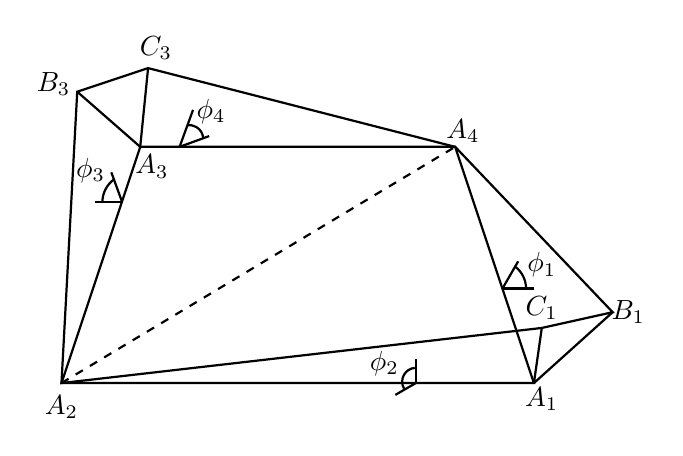
\begin{tikzpicture}[>=latex]           %   \draw[help lines] (0,0) grid (15,10);

        \coordinate (a1) at (9, 4);
        \coordinate (a2) at (3, 4);
        \coordinate (a3) at (4, 7);
        \coordinate (a4) at (8, 7);
        \coordinate (b1) at (10, 4.9);
        \coordinate (c1) at (9.1, 4.7);
        \coordinate (b2) at (2.3, 3);
        \coordinate (c2) at (2.15, 4.3);
        \coordinate (b3) at (3.2, 7.7);
        \coordinate (c3) at (4.1, 8);
        \coordinate (b4) at (7.9, 8);
        \coordinate (c4) at (9, 7.5);

        \draw[thick] (a1) -- (a2) -- (a3) -- (a4) -- cycle;
        
        \draw[dashed, thick] (a2) -- (a4);
        
        
        \draw[thick] (b1) -- (c1) -- (a2) -- (b3) -- (c3) -- (a4) -- cycle;
        
        \draw[thick] (a1) -- (b1);
        \draw[thick] (a1) -- (c1);
    
        \draw[thick] (a3) -- (b3);
        \draw[thick] (a3) -- (c3);

        \draw (a1) + (0.1, -0.2) node {$A_1$};
        \draw (b1) + (0.2, 0) node {$B_1$};
        \draw (c1) + (0, 0.25) node {$C_1$};
        
        \draw (a2) + (0, -0.3) node {$A_2$};
        
        \draw (a3) + (0.15, -0.25) node {$A_3$};
        \draw (b3) + (-.3, 0.1) node {$B_3$};
        \draw (c3) + (0.1, .25) node {$C_3$};
        
        \draw (a4) + (0.1, 0.2) node {$A_4$};
        
        \draw[thick] (7.5, 4) -- (7.5, 4.3);
        \draw[thick, rotate around = {30:(7.5, 4)}] (7.5, 4) -- (7.2, 4);
        \draw[thick] (7.35, 3.93) arc (210:95:5pt);
        \draw (7.1, 4.25) node {$\phi_2$};
        
        \draw[thick] (8.6, 5.2) -- (9, 5.2);
        \draw[thick, rotate around = {60:(8.6, 5.2)}] (8.6, 5.2) -- (9, 5.2);
        \draw[thick] (8.9, 5.2) arc (0:51:10pt);
        \draw (9.1, 5.5) node {$\phi_1$};

        \draw[thick, rotate around = {20:(4.5, 7)}] (4.5, 7) -- (4.9, 7);
        \draw[thick, rotate around = {70:(4.5, 7)}] (4.5, 7) -- (5, 7);
        \draw[thick] (4.8, 7.1) arc (0:100:5pt);
        \draw (4.9, 7.45) node {$\phi_4$};

        %\draw (3.75, 6.3) node {\textbullet};
        \coordinate (phi3) at (3.77, 6.3);
        \draw[thick, rotate around = {-70:(phi3)}] (phi3) -- + (-0.4,0);
        \draw[thick] (phi3) -- + (-0.35, 0);
        \draw[thick] (phi3) + (-0.25, 0) arc (180:125:10pt);
        \draw (phi3) + (-0.4,0.4) node {$\phi_3$};
        
     \end{tikzpicture}